\section{Set theory and logic}
\label{set-theory}
The theory of sets, typically referred to as \word{set theory}{m{\"a}ngdteori}, forms the basic fundament of all of mathematics. As such, it is probably unsurprising that a huge body of work has been devoted to it. This, however, is not obvious if one simply reads these notes as we will not at all deal with many of the important ideas that underly the theory. Moreover, even though set theory plays an essential role in our study, our treatment of set theory will be rather brief, so the inexperienced reader is also strongly encouraged to study \cite[\S1]{Mun} in detail.

\subsection{Basic notions}
Whereas everything that we will during the course will be as mathematically precise as one can get, we will begin by imprecisely considering a \word{set}{m{\"a}ngd} as a ``collection of things'' (formally, we require a set to satisfy the ZFC axioms but we will not list those here\footnote{The interested reader can find the axioms at \url{https://en.wikipedia.org/wiki/ZFC}.}). These ``things'' will be referred to as the \emph{elements} of the set.

If $A$ is a set, and $a$ is an element of $A$, we write
\[
  a \in A.
\]
Synonymously, we will sometimes say that $a$ is contained in $A$. If on the other hand $a$ is not an element of $A$, then we write
\[
  a \notin A.
\]
If $B$ is another set which contains all the elements of $A$; that is, if $a \in A$ implies that $a \in B$, then we say that $A$ is a \word{subset}{delm{\"a}ngd} of $B$ and write
\[
  A \subset B.
\]
We will also sometimes say that $A$ is contained in $B$ or that $B$ contains $A$. If $A \subset B$ but $A \not= B$, we will write
\[
  A \subsetneq B
\]
and say that $A$ is a \word{proper subset}{{\"a}kta delm{\"a}ngd} of $B$. Set-theoretic relationships are often depicted in so-called Euler diagrams; see Figure~\ref{eulersubset}.
\begin{figure}
  \centering
  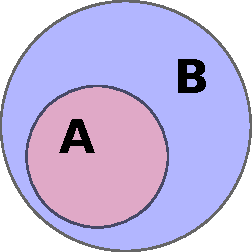
\includegraphics{images/subset.pdf}
  \caption{The Euler diagram representing the inclusion $A \subset B$.}
  \label{eulersubset}
\end{figure}
\begin{example}
  When a set contains only very few elements, one simply lists them. For instance, if $A$ contains only the elements $a$ and $b$, we write $A = \{ a, b\}$. Then if $B = \{ a, b, c\}$, we see for instance that $A \subset B$ and since $c \in B$ but $c \notin A$, we have that $A \not= B$, so $A \subsetneq B$.
  
  Often, sets are given by the properties of their elements, and this will be built into our notation. For instance, the set containing the even numbers will be written
  \[
    \{ x \mid \text{$x$ is an even integer} \},
  \]
  which should be read as ``$x$ such that $x$ is an even integer''.
  
  We will also often be considering the set which contains no elements at all; this set is called \wordexp{the empty set}{den tomma m{\"a}ngden}{empty set, the}{den tomma m{\"a}ngden} and is denoted $\emptyset$. This has the property that $\emptyset \subset X$, no matter what $X$ is.
\end{example}
\begin{defn}
  Let $X$ be any set. The \word{power set}{potensm{\"a}ngd} of $X$, denoted $\calP(X)$ is the set of all subsets of $X$, that is
  \[
    \calP(X) = \{U \mid U \subset X \}.
  \]
\end{defn}
\begin{example}
  The elements of power sets are themselves sets which in turn may also have elements. Some examples of power sets are the following:
  \begin{align*}
    \calP(\{a\}) &= \{ \emptyset, \{a \} \}, \\
    \calP(\{a,b\}) &= \{ \emptyset, \{a\}, \{b\} , \{a,b\} \}.
  \end{align*}
  In general, if $X$ is a finite set containing $n$ elements, then $\calP(X)$ contains $2^n$ elements. The only subset of $\emptyset$ is $\emptyset$ itself, which means that
  \[
    \calP(\emptyset) = \{\emptyset\}.
  \]
  Be aware that $\{ \emptyset \}$ consists of a single element, namely $\emptyset$, so $\{\emptyset\}$ is not itself empty, even though it is tempting to read the notation like that.
\end{example}
\trans{intersection}{snitt}\trans{disjoint}{disjunkt}\trans{difference}{differens}\trans{complement}{komplement}
\begin{defn}
  Given two sets $A$ and $B$, we define their \word{union}{union} $A \cup B$ and \word{intersection}{snitt} $A \cap B$ as
  \begin{align*}
    A \cup B &= \{ x \mid \text{$x \in A$ or $x \in B$} \}, \\
    A \cap B &= \{ x \mid \text{$x \in A$ and $x \in B$} \}.
  \end{align*}
  The sets $A$ and $B$ are called \word{disjoint}{disjunkt} if $A \cap B = \emptyset$. We also introduce the \word{difference}{differens} $A \setminus B$, or sometimes $A - B$, given by
  \[
    A \setminus B = \{ x \mid \text{$x \in A$ and $x \notin B$} \}.
  \]
  If $A \subset X$ for some set $X$, we introduce the \word{complement}{komplement} of $A$, written $A^c$ as
  \[
    A^c = X \setminus A.
  \]
  Note that $X$ does not feature in the notation for complements but which set it is will always be clear from the context. See Figure~\ref{union-intersection} for the corresponding Euler diagrams.
\end{defn}
\begin{figure}
  \centering
  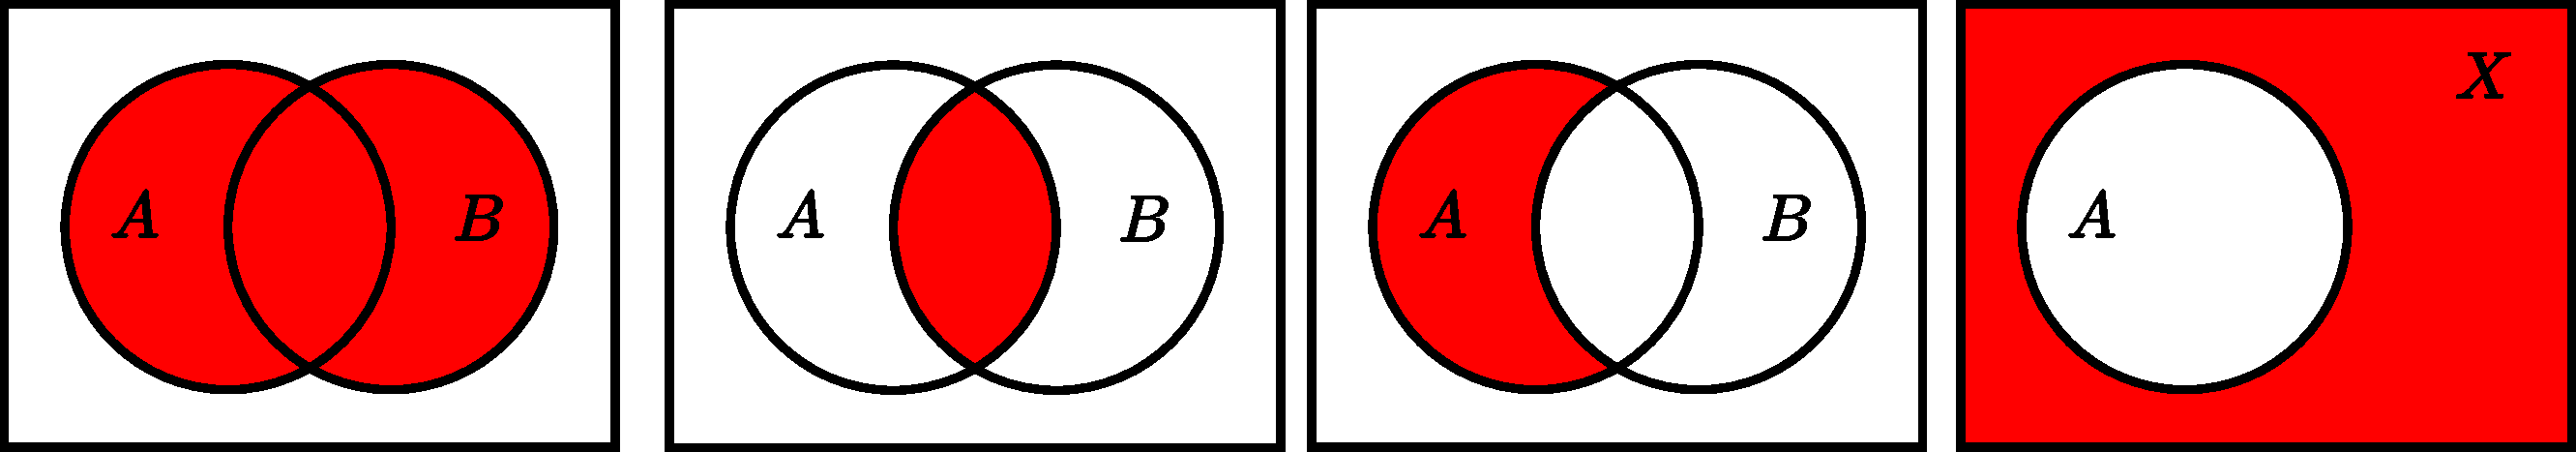
\includegraphics[scale=0.3]{images/union-intersection.pdf}
  \caption{The red sets illustrate $A \cup B$, $A \cap B$, $A \setminus B$, and $A^c$ respectively.}
  \label{union-intersection}
\end{figure}

\subsection{Set theory and boolean logic}
At this point, let us remark that sets and their operations closely mimic logical statements and their boolean logic, and without making this statement too precise, one could summarize their relationship in the following table:

\begin{center}
\begin{tabular}{ccc}
  logic & English & set theory \\
  \hline
  $P \Rightarrow Q$ & $P$ implies $Q$ & $A \subset B$ \\
  $P \Leftrightarrow Q$ & $P$ is equivalent to $Q$ & $A = B$ \\
  $P \vee Q$ & $P$ or $Q$ & $A \cup B$ \\
  $P \wedge Q$ & $P$ and $Q$ & $A\cap B$ \\
  $\neg P$ & not $P$ & $A^c$
\end{tabular}
\end{center}

For convenience, and for those who may not have encountered boolean logic before, we recall that these logical operations are defined through truth tables. Here, $P$ and $Q$ are statements that may be either true (T) or false (F), and the values of $P \Rightarrow Q$, $P \Leftrightarrow Q$, etc., are defined accordingly:
\begin{center}
\begin{tabular}{c|c}
  $P$ & $\neg P$ \\
  \hline
  T & F \\
  F & T
\end{tabular}
\quad \quad
\begin{tabular}{cc|cc}
  $P$ & $Q$ & $P \wedge Q$ & $P \vee Q$ \\
  \hline
  T & T & T & T \\
  T & F & F & T \\
  F & T & F & T \\
  F & F & F & F
\end{tabular}
\end{center}

In these tables, the columns to the left of the vertical bar are the assumptions, and the columns to the right are the definitions. Armed with these definitions, one simply defines $P \Rightarrow Q$ as $\neg P \vee Q$, and similarly $P \Leftrightarrow Q$ is defined as $(P \Rightarrow Q) \wedge (Q \Rightarrow P)$.

With these, one sees that the correspondence in the first table in this section is obtained when $P$ is the statement $a \in A$, and $Q$ is the statement $a \in B$.

\subsection{Arbitrary unions and intersections}
So far, we have considered only operations on pairs of sets, but more often than not we will be dealing with infinite families of sets. First of all, we introduce the notation $\forall$ meaning ``for all'', and $\exists$ meaning ``there exists''.

Let $I$ be any set. Then a collection $\{ A_i \}_{i \in I}$ of sets $A_i$ is called a family of sets parametrised by $I$. For such a family, define the infinite union, and the infinite intersection as
\begin{align*}
  \bigcup_{i \in I} A_i &= \{ x \mid \text{$\exists i \in I$ such that $x \in A_i$} \},\\
  \bigcap_{i \in I} A_i &= \{ x \mid \text{$x \in A_i \ \forall i \in I$} \}.
\end{align*}
It might be helpful to compare these definitions with the definitions of union and intersection from above, which is the case where $I$ contains two elements.

\begin{prop}
  \label{de-morgan}
  For sets $A$, $B$, $C$, and $X$, for a family $\{ A_i \}_{i \in I}$ with $A_i \subset X$ for all $i \in I$, one has the useful identities,
  \begin{align*}
    A \cap (B \cup C) &= (A \cap B) \cup (A \cap C), \\
    A \cup (B \cap C) &= (A \cup B) \cap (A \cup C), \\
    X \setminus \bigcup_{i \in I} A_i &= \bigcap_{i \in I} X \setminus A_i, \\
    X \setminus \bigcap_{i \in I} A_i &= \bigcup_{i \in I} X \setminus A_i.
  \end{align*}
  Various versions of these equalities are known as \emph{De Morgan's laws}\index{De Morgan's laws}.
\end{prop}
\begin{proof}[Partial proof]
  Set theoretical identities like the above are typically shown in the same way: one starts with an element in the left hand side and proves that it is an element of the right hand side, which shows ``$\subset$'', and one then proceeds to do the same thing the other way around. To convince oneself that the identities indeed hold, it may be helpful to draw the corresponding Euler diagrams.
  
  Let us show for instance that $A \cap (B \cup C) \subset (A \cap B) \cup (A \cap C)$. To do this, let $a \in A \cap (B \cup C)$. This means that $a \in A$ and $a \in B \cup C$. The latter of these means that $a \in B$ or $a \in C$. Together, this says that either $a \in A$ and $a \in B$, or $a \in A$ and $a \in C$. Written in set notation, this says that $a \in (A \cap B) \cup (A \cap C)$.
  
  Let us also show that $X \setminus \bigcup_{i \in I} A_i \subset \bigcap_{i \in I} X \setminus A_i$. That is, let $a \in X \setminus \bigcup_{i \in I} A_i$. This says that $a \notin \bigcup_{i \in I} A_i$. From this we conclude that $a$ is not in any of the $A_i$ (since otherwise $a$ would be in their union), or in symbols, $\forall i \in I$, we have $x \notin A_i$. That is, $\forall i \in I$, we have $x \in X \setminus A_i$, but this exactly means that $x \in \bigcap_{i \in I} X \setminus A_i$.
  
  We leave the remaining six directions for the reader.
\end{proof}

\subsection{Cartesian product}
\label{cartesian-product}
Another way of constructing new sets from old sets is through the so-called Cartesian product, often simply called a product. In words, if $A$ and $B$ are two sets, then the \word{Cartesian product}{kartesisk produkt} $A \times B$ is the set of all pairs $(a,b)$, where $a \in A$, or $b \in B$; that is,
\[
  A \times B = \{ (a,b) \mid \text{$a \in A$ and $b \in B$}\}.
\]
Be aware that $(a,b)$ is occasionally used as the notation for intervals of real numbers, but this is something completely different.

\begin{example}
  One way of defining $\bbR^2$ is simply as $\bbR^2 = \bbR \times \bbR$.
\end{example}
Just as for unions and intersections, we would like to be able to talk about infinite products. A little bit of care needs to be taken when defining these. For instance, what is $X \times Y \times Z$? There are two natural definitions: $(X \times Y) \times Z$ and $X \times (Y \times Z)$. The first set consists of elements of the form $((x,y),z)$, while the second one consists of elements of the form $(x,(y,z))$. Clearly, we should be able to think of any of these as simply triples $(x,y,z)$.

To make this precise for an infinite number of sets, consider a family $\{X_i \}_{i \in I}$. The infinite product should then consist of tuples $(x_i)_{i \in I}$ with $x_i \in X_i$ for all $i$. Such a tuple we can also view as a function $x : I \to \bigcup_{i \in I} X_i$ such that $x(i) \in X_i$ for all $i$. This brings us to the following.
\begin{defn}
  The Cartesian product of a family $\{X_i \}_{i \in I}$ is the set
  \[
    \prod_{i \in I} X_i = \left\{ x : I \to \bigcup_{i \in I} X_i \relmiddle| x(i) \in X_i \ \forall i \in I \right\}.
  \]
\end{defn}

\subsection{Relations}
Above, we have talked about various relations between sets; these we will now make mathematically precise. A \word{binary relation}{bin{\"a}r relation} $C$, often simply called a \word{relation}{relation}, on a set $A$ is a subset $C \subset A \times A$. When $(x,y) \in C$, we will often write $xCy$.

\begin{example}
  \label{example-inequality}
  The subset of $\bbR \times \bbR$ given by $C = \{(x,y) \mid x \leq y\}$ is a relation on $\bbR$, and $xCy$ if and only if $x \leq y$.
\end{example}

\trans{reflexive}{reflexiv}\trans{symmetric}{symmetrisk}\trans{anti-symmetric}{antisymmetrisk}\trans{transitive}{transitiv}\trans{total}{total}
\begin{defn}
  A relation $C \subseteq A \times A$ is called
  \begin{itemize}
    \item \word{reflexive}{reflexiv} if $xCx$ for all $x \in A$,
    \item \word{symmetric}{symmetrisk} if $xCy$ implies that $yCx$ for all $x,y \in A$,
    \item \word{anti-symmetric}{antisymmetrisk} if $xCy$ and $yCx$ implies that $x = y$ for all $x, y \in A$,
    \item \word{transitive}{transitiv} if $xCy$ and $yCz$ implies that $xCz$ for all $x,y,z \in A$,
    \item \word{total}{total} if either $xCy$ or $yCx$ when $x, y \in A$.
  \end{itemize}
\end{defn}
\begin{example}
  The relation $\leq$ from Example~\ref{example-inequality} is reflexive, anti-symmetric, transitive, and total, but it is not symmetric.
\end{example}
\trans{partial order}{partiell ordning}
\begin{defn}
  \label{def-poset}
  A relation $C$ on a set $A$ is called a \word{partial order}{partiell ordning} if it is reflexive, anti-symmetric, and transitive. The pair $(A,C)$ is called a \word{poset}{pom{\"a}ngd}. If the partial order relation is also total, then it is called a \emph{total order}\index{total order}, and $(A,C)$ is called a \emph{totally ordered set}\index{totally ordered set}
\end{defn}
We will often denote partial orders by the symbol $\preceq$.
\trans{poset}{pom{\"a}ngd}\trans{equivalence relation}{ekvivalensrelation}
\begin{defn}
  An \word{equivalence relation}{ekvivalensrelation} is a relation which is reflexive, symmetric, and transitive.
\end{defn}
When $C$ is an equivalence relation, we will use the notation $x \sim y$ for $xCy$ and say that $x$ is equivalent to $y$.
\begin{example}
  \label{congruence}
  Fix a positive integer $p \in \bbN$, and let $C \subset \bbZ \times \bbZ$ be the subset of pairs $(m,n)$ such that $m-n$ is a multiple of $p$, i.e. $m-n = dp$ for some $d \in \bbZ$. This is an equivalence relation.
\end{example}
Given any equivalence relation on a set $A$, it is possible to partition $A$ into smaller sets consisting of elements that are equivalent to each other. More precisely, for $x \in A$, let
\[
  [x] = \{ y \mid y \sim x \}
\]
be the so-called \word{equivalence class}{ekvivalensklass} of $x$. Note that $x \sim x$ by reflexivity so $x \in [x]$ for all $x \in A$.
\begin{lem}
  Let $\sim$ denote an equivalence relation on a set $A$. For two elements $x, x' \in A$, the equivalence classes $[x]$ and $[x']$ are either disjoint or equal.
\end{lem}
\begin{proof}
  Suppose that $[x]$ and $[x']$ are not disjoint and let us show that they must then be equal. That is, let $y \in [x]$ be arbitrary, and let us show that $y \in [x']$. Since $[x]$ and $[x']$ are not disjoint, there is a $z \in A$ such that both $z \in [x]$ and $z \in [x']$. That is, $z \sim x$, and $z \sim x'$. Since $y \in [x]$ we have $y \sim x$, so by symmetry, $x \sim y$, and by transitivity, $z \sim y$. Thus by symmetry, $y \sim z$, and by transitivity $y \sim x'$, but this says that $y \in [x']$. This shows that $[x] \subset [x']$. By the exact same argument one shows that $[x'] \subset [x]$ so that $[x] = [x']$.
\end{proof}
The set of equivalence classes on a set $A$ with respect to an equivalence relation $\sim$ will be denoted $A/\!\sim$. That is,
\[
  A/\!\sim = \{ [x] \mid x \in A \}.
\]
\begin{example}
  Consider the relation $\sim$ from Example~\ref{congruence}. The equivalence class of an integer $n \in \bbZ$ is the set of integers
  \[
    [n] = \{\dots, n-2p, n-p, n, n+p, n+2p, \dots \},
  \]
  and we can write $\bbZ$ as the union of $p$ equivalence classes, as
  \[
    \bbZ = [0] \cup [1] \cup [2] \cup \dots \cup [p-1].
  \]
  Similarly,
  \[
    \bbZ/\!\sim = \{[0], [1], \dots, [p-1]\}.
  \]
\end{example}
